\section{Performance}
\subsection{Performance measurement introduction}
Before a performance measurement or comparison between database systems can be made, it is necessary to define the performance indicators. Depending on the use-case of the measured databases the results can be completely different. For example a real-time system is a lot more dependent on access times, latency and fast updates for concurrent users. A scientific database has to be fast at processing complex queries with joints and preprocessing routines like aggregation \cite{Neil_O}. Of course the benchmark should be implemented to test the performance of a database system in a way that reflects your usage in the future.
\\\\
For database systems there is a council called the TPC . This organization tests different database systems on physical and virtual machines and scores them by performance. The performance indicators can be seen on their website and there are different benchmarks depending on the use-case of the system \cite{_tpc.org.}. 
\\\\
Another standardized benchmark for database implementations is the Wisconsin Benchmark. This was one of the first standardized benchmarks and was made for relational databases. The test contains of inserts, selections, joints and projections. For further details on this benchmark, see the paper \cite{DeWitt_The_1991}.
\\\\
This paper will summarize MonogDB performance compared to other popular NoSQL and SQL  databases.

\subsection{Influencing factors to database performance}
All the results provided by this paper are dependent on the underlying hardware used. Depending on the host system for the database application, the performance can vary a lot \cite{Lee_W._2009}. Examples for big performance factors are available memory, processor speed and the used storage.
\\\\
For evaluation which database system should be used, it is important to know on what kind of hardware the production system will run. This is due to the fact, that different database systems were developed to meet certain performance goals on different hardware. Therefore some databases scale well with more memory and memory bandwidth since they try to cache a lot of the data in system memory. But there are also databases which try to be very lightweight on memory for low end systems or massive I/O  operations \cite{Boncz_Database_1999}.
\\\\
Nearly all databases are reliant on the used storage. This storage is the only way to keep the data, even when the system is turned off. Even In-memory databases use the persistent storage to save their current data \cite{Wang_Main_2001}. As transactions ultimately have to be written to the storage, this becomes the biggest bottleneck. With traditional HDDs having a high latency when accessing random data, which happens frequently on a database system, the introduction of SSDs  eliminated those problems. Benchmarks done on traditional HDD storage can be translated most of the time to SSDs since all databases will perform better but should stay at the same relative performance.
\subsection{NOSQL compared to SQL databases}
It is often one of the first question, when talking about database performance. SQL or NOSQL, which one is faster? Comparing those two types of databases generally, is not really useful. The way how data is stored is completely different and the use-case defines if SQL or NOSQL fits better.
\\\\
A good example for the difference of these two types is Twitter. They use a NOSQL database for all the tweets. Although Twitter is using MySQL heavily. The reason for this is easy to explain. A tweet contains some sort of content like text or images and a lot of additional information like hashtags, user and topics. Storing that data in a relational, normalized way, it would take a lot of tables and joins to represent a tweet . All hashtags would be referenced over multiple tables. These joins take time and since Twitter is a real time platform, latency should be low \cite{Weil_21}.
\\\\
In contrast the NOSQL implementation is way easier. The complete Tweet is stored as a document. The hashtags and links are stored in the same document in a key value manner. Now when you want to read 100 Tweets, in a NOSQL context, this can be done by one simple query. In a relational model, complex joins for each Tweet would be necessary. In such a scenario performance is obviously on the NOSQL side, but only because the use-case is well suited for non-relational models.
\subsection{MongoDB performance}
This paper will be limited to benchmarks of low level functions for databases. These functions are: reads, writes and deletions. Performance is measured between MongoDB and MariaDB. MariaDB is a SQL database and as previously mentioned, general comparisons between NOSQL and SQL are not useful. In this case two implementations of SQL and NOSQL are compared which is relevant when the use-case can be implemented by both designs without drawbacks. In such a scenario, raw performance is a valid factor.
In addition to the benchmark implemented by the author of this section, another one is used for validity and a broader overview. The referenced paper contains additional databases.
\\\\
The following performance test were performed, using NodeJS. For MongoDB connectivity the official MongoDB driver  was used. The same applies for the MariaDB driver . The driver selection can cause huge performance differences. There are several MariaDB drivers for NodeJS and of course other programming languages. Therefore comparisons of database performance should be done, using the same programming language \cite{_mscdex.}. The inserted data contains just an id represented by an integer.
\begin{figure}[H]
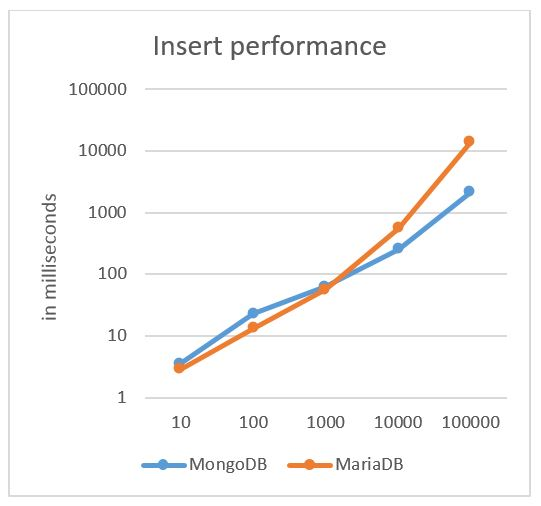
\includegraphics[width=\linewidth,keepaspectratio]{images/Performance_Inserts.JPG}
\caption{Insert MongoDB vs MariaDB}
\label{arch-example}
\end{figure}
\begin{figure}[H]
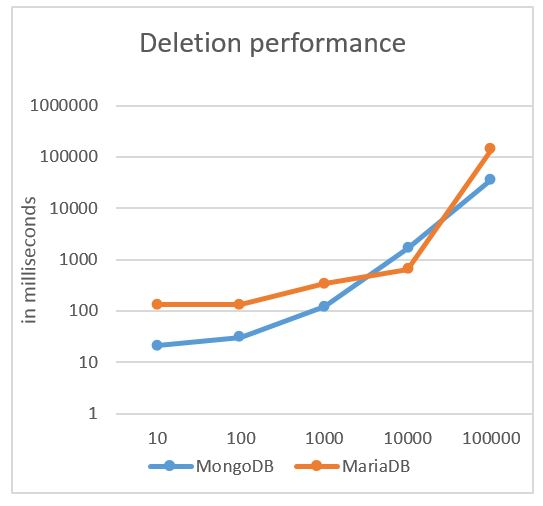
\includegraphics[width=\linewidth,keepaspectratio]{images/Performance_Deletion.JPG}
\caption{Deletion performance}
\label{arch-example4}
\end{figure}

The numbers show an interesting result. In the insert test MongoDB performs worse than MariaDB just slightly up to the point of 1000 inserts. After that point MariaDB falls behind. With increasing number of inserts the performance leap of MongoDB increases a lot. A reason for this could be some kind of overhead for inserts on MongoDB, further investigation is needed to evaluate the results and the cause. A similar behavior can be seen on deletion test.
\\\\
The following performance results are provided by the paper \cite{Li_A_2013}
\begin{figure}[H]
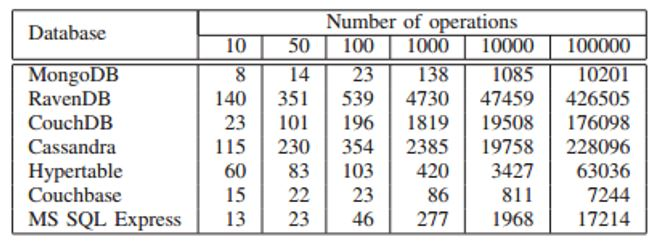
\includegraphics[width=\linewidth,keepaspectratio]{images/Performance_Reads.JPG}
\caption{time for read operations in milliseconds}
\label{arch-example2}
\end{figure}
\begin{figure}[H]
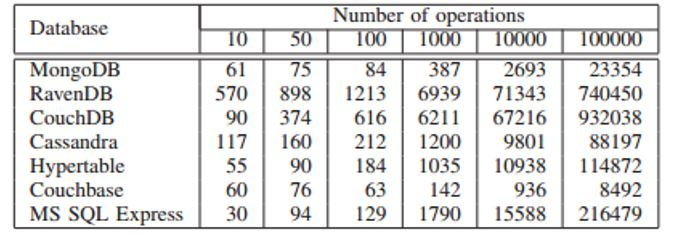
\includegraphics[width=\linewidth,keepaspectratio]{images/Performance_Writes.JPG}
\caption{time for write operation in milliseconds}
\label{arch-example3}
\end{figure}
\begin{figure}[H]
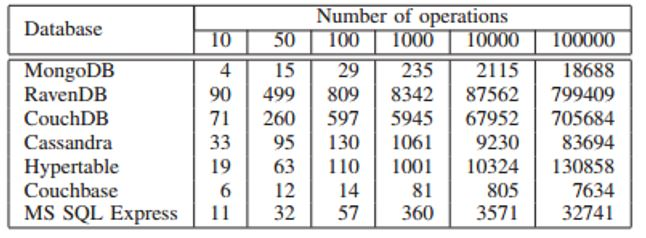
\includegraphics[width=\linewidth,keepaspectratio]{images/Performance_Delete.JPG}
\caption{time for delete operation in milliseconds}
\label{arch-exampl1}
\end{figure}

Interestingly the benchmarks from the paper show similar results on write performance when comparing the SQL implementation and MongoDB. After 100 writes MongoDB performs better. When comparing to other NoSQL databases, MongoDB is always in the upper half of the field. So it can be said, that this database should be suited well for demanding applications and performance shouldn't be a major problem. 
\\\\
These statements only apply for single instance usage. Since MongoDB uses a single master architecture for multiple instances, throughput will be less than database systems that trade consistency for performance. Using sharded servers can increase performance for horizontal scaling. With this addition, MonngoDB is also very usable for scientific applications with high amounts of I/O and data \cite{Dede_Performance_2013}.



